\documentclass[onecolumn,12pt]{IEEEtran}
\usepackage[utf8]{inputenc}
\usepackage[left=1in,right=1in,bottom=0.95in,nohead,nofoot]{geometry}
\usepackage{graphicx}

\begin{document}
\title{Informe Laboratorio 5}
\author{Redes de Datos}
%\vspace{3mm}

\begin{figure}[h]

\includegraphics[width=0.50\textwidth]{logo_udp.png}
\label{fig:mesh1}
\\
\\
\\
\\
\\
\maketitle
\end{figure}
\begin{center}
Integrantes:\\
\hfill \\
Gonzalo Felipe\\
Andres Hernandez\\
Franco Centeno\\
\hfill \\
\hfill \\
\hfill \\
\hfill \\
\ \hfill \\
Profesor:\\
Jose Perez\\ \hfill \\
Ayudante:\\
Alexis Inzunza\\
\end{center}

\newpage
\title{Indice}
\author{ }
\maketitle
\hrule
\tableofcontents

\newpage
\section{INTRODUCCION}
\hfill \\

En este laboratorio trabajamos con el protocolo STP (Spanning Tree Protocol) el cual es un protocolo de la capa dos del modelo OSI (Enlace de Datos), que se ejecuta en switches como bridges. El objetivo de este protocolo es garantizar que se impida la creación de bucles en vias redundantes en la red, ya que los bucles son fatales en una red.

\hfill \\
\section{ACTIVIDAD}
\hfill \\

La actividad I consiste en analizar los problemas que ocurren cuando una topología de red presenta enlaces redundantes y se crean bucles, para luego analizar la misma topología incorporando el protocolo STP para ver sus ventajas en cuanto a la redundancia y robustez de la LAN. Para esta actividad debe utilizar la siguiente topología:

\begin{figure}[!h]
\centering
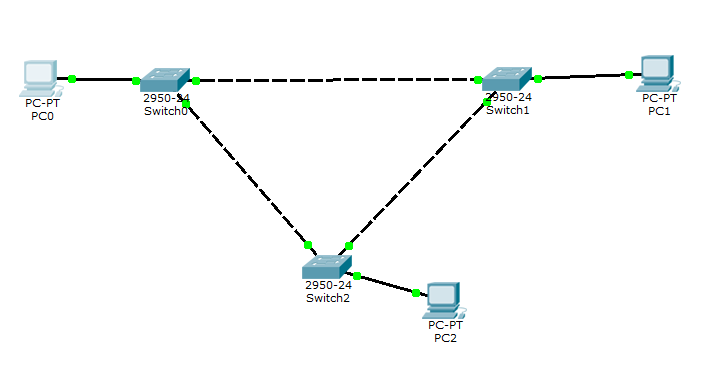
\includegraphics[width=0.7\textwidth]{top1.PNG}
\label{fig:mesh1}
\end{figure}

La actividad II se trabaja con la misma topología de la actividad I, configurando el switch 1 como primario y otro switch como secundario aplicando comandos en la configuración de los switches.\\

En la actividad III se debe asignar prioridades a los switches para analizar el comportamiento del protocolo STP con respecto a las prioridades asignadas.\\

\newpage

Por último, en la actividad IV se vera la configuración de diferentes dispositivos involucrados en la implementación de VLANs. Se comienza con la configuración del switch con cuatro VLANs estáticas y luego con los demás switches, para poder comunicar entre si las diferentes VLANs, simulando que cada una de las VLANs se encuentran en pisos distintos.

\begin{figure}[!h]
\centering
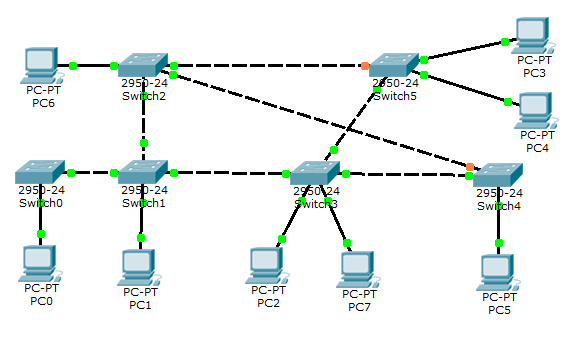
\includegraphics[width=0.7\textwidth]{top2.PNG}
\label{fig:mesh1}
\end{figure}

\section{CUESTIONARIO}
\hfill \\
(ACTIVIDAD I) ¿Qué camino realizara un paquete que para llegar desde el switch 0 hasta el
switch 2?\\ \\
R: Sin el protocolo STP activado, se manda el paquete a todas direcciones, creando un bucle sin fin. Con el protocolo activado se envia hacia el switch 1, pero luego comienza un bucle otra vez.
\\ \\
(ACTIVIDAD I) ¿Qué camino realizara un paquete que para llegar desde el switch 2 hasta el
switch 1?\\ \\
R: Sin el protocolo STP activado, se envia el paquete al switch 1 y llega, pero luego comienza un bucle con otro paquete entre los switches. Con el protocolo activado, se envia directamente al switch 1, llega el paquete exitosamente.
\\ \\
(ACTIVIDAD II) ¿Qué camino realizara un paquete que para llegar desde el switch 2 hasta el
switch 0?\\ \\
R: Primero se va hacia el switch primario, el cual es el switch 1, y luego va hacia el switch 0, para entregarse exitosamente y luego pasa por el switch primario y de vuelta hacia el 2 para recibirse exitosamente.
\\ \\
(ACTIVIDAD II) ¿Qué camino realizara un paquete que para llegar desde el switch 1 hasta el
switch 0?\\ \\
R: Se va directamente al switch 0, para llegar exitosamente, y luego directamente al switch 1 para recibirse exitosamente.
\\ \\
(ACTIVIDAD IV) ¿Cuál es la diferencia del modo Access y el modo Trunk en un switch?\\ \\
R: El modo Trunk permite manejar el tráfico de distintas VLANs en un mismo puerto, cada paquete se etiqueta. Se utiliza para interconectar distintos tipos de equipos de red, como por ejemplo un par de switches. El modo Access solo permite pasar solo una vlan, los paquetes no se etiquetan, y generalmente es usado para conectar dispositivos finales.
\\ \\
(ACTIVIDAD IV) ¿Qué ocurre si conecto una puerta en modo Trunk a un PC?\\ \\
R: El host, el PC que está conectado en este caso, puede recibir paquetes de multiples VLANs, probablemente este PC puede llegar a inundarse de información.
\\ \\
(ACTIVIDAD IV) ¿Qué ocurre si conecto dos switches, uno en modo access y otro en modo trunk?\\ \\
R: El switch en modo access solo transportaría paquetes de una sola VLAN
\\ \\
(ACTIVIDAD IV) ¿Qué camino realizara un paquete que para llegar desde el switch 1 hasta el switch 0?\\ \\
R: Primero se va hacia el switch 1, y luego va hacia el switch 0, para entregarse exitosamente y luego pasa por el switch 1 y de vuelta hacia el 2 para recibirse exitosamente.

\newpage
\section{CONCLUSION}
\hfill \\

Hoy en día, el rendimiento de la red puede llegar a ser un factor en la productividad de una organización, es vital una buena comunicación entre los equipos para lograr un mejor rendimiento. Es por esto que la utilización del protocolo STP es fundamental, como también lo son las distintas VLAN, así se puede llegar a lograr una red segura y ordenada, organizando bien las conexiones de cada red.



\hfill \\
\hfill \\
\section{BIBLIOGRAFIA}
\hfill \\
Modo Access y Modo Trunk,
\emph{NKSistemas} \\
\url{https://nksistemas.com/parte-13-puerto-en-modo-access-vs-trunk/}


\end{document} 
